\documentclass[a4print,italian,lof,lot,oneside]{univpmthesis}
\errorcontextlines=9
\RequirePackage[utf8]{inputenc}
\RequirePackage[T1]{fontenc}
\usepackage{lmodern}

%%%%%%%%%%%%%%%%%%%%%%%%%%%%%%%%%%%%%%%%%%%%%%%%%%%%%%%%%%%
% Metadata
%%%%%%%%%%%%%%%%%%%%%%%%%%%%%%%%%%%%%%%%%%%%%%%%%%%%%%%%%%%
\thfaculty{Facolt\`{a} di Ingegneria}
\thcourse{Corso di Laurea in Ingegneria Informatica e dell'Automazione}
\thtitle{Sviluppo e porting di firmware per drone di tipo Ducted Fan}
\thsubtitle{Sottotitolo della Tesi}
\thauthor{Robert Laurentiu Mincu}
\thadvisor{Andrea Bonci}
\thcoadvisor{Prof.~Nome Correlatore 1}{Prof.~Nome Correlatore 2}{}

\ayear{2024-2025}

\thesisdedication{La dedico a Giada, Alina e Paolo}
\thlocation{Ancona}
\thtime{Dal 1/2/2025 al 1/10/2025} % data scrittura
%%%%%%%%%%%%%%%%%%%%%%%%%%%%%%%%%%%%%%%%%%%%%%%%%%%%%%%%%%%

\usepackage{amsmath,amsfonts,amssymb,bm} %<- scrittura equazioni
\usepackage{graphicx} 	%<- immagini
\usepackage{epstopdf} 	%<- conversione immagini .eps
\usepackage{subfig} 	%<- sottofigure
\usepackage{footnote}	%<- note a piè pagina
\usepackage{tabularx,booktabs,multicol,multirow} %<- tabelle
\usepackage{mathrsfs}
\usepackage{caption}	%<- didascalie
\usepackage{microtype}
\usepackage{gensymb,siunitx}	%<- simboli ed unità di misura
\usepackage{hyperref}   %<- link
\usepackage{glossaries}
\usepackage{verbatim}
\usepackage{xcolor}
\usepackage[a-1b]{pdfx} %<- generazione pdf-A
\usepackage{listings}   %<- per inserire il codice

%%%%%%%%%%%%%%%%%%%%%%%%%%%%%%%%%%%%%%%%%%%%%%%%%%%%%%%%%%%
\newcommand{\eqname}{Eq.}
%%%%%%%%%%%%%%%%%%%%%%%%%%%%%%%%%%%%%%%%%%%%%%%%%%%%%%%%%%%%%%%%%%%%
\definecolor{custom_green}{rgb}{0,0.6,0}
\definecolor{codegray}{rgb}{0.5,0.5,0.5}
\definecolor{codepurple}{rgb}{0.58,0,0.82}
\definecolor{backcolour}{rgb}{0.95,0.95,0.92}
\definecolor{custom_blue}{rgb}{  0.05, 0.05, 0.97}
\definecolor{custom_brown}{rgb}{ 0.69, 0.38, 0.10}
\definecolor{custom_purple}{rgb}{0.58, 0.00, 0.82}
\definecolor{custom_orange}{rgb}{0.94, 0.59, 0.09}

\lstdefinelanguage{Cpp}{
    language=C++,
    backgroundcolor=\color{white},
    basicstyle=\footnotesize\ttfamily\color{black},
    breakatwhitespace=false,
    breaklines=true,
    captionpos=b,
    morecomment=[l]{//},
    morecomment=[s]{/*}{*/},
    morestring=[b]{"},
    commentstyle=\color{custom_green},
    morekeywords={int, char, do, while, for, strtok, strtof, NULL, free, const, float},
    sensitive=false,
    keywordstyle=\color{custom_purple},
    stringstyle=\color{blue},
    numbers=left,
    numbersep=5pt,
    numberstyle=\tiny\color{black},
    rulecolor=\color{black},
    showspaces=false,
    showstringspaces=false,
    showtabs=false,
    stepnumber=1,
    tabsize=4,
    title=\lstname
}

\lstdefinelanguage{Python}{
    keywords={from, import, def, return, as, in, len, if, elif, else, for, while, self},
    breakatwhitespace=false,       
    breaklines=true,   
    morecomment=[l]{\#},
    morestring=[b]",
    commentstyle=\color{red},
    keywordstyle=\color{custom_purple},
    numberstyle=\tiny\color{black},
    stringstyle=\color{custom_green},
    basicstyle=\ttfamily\footnotesize,
    captionpos=b,
    showstringspaces=false,        
    showtabs=false,                
    numbers=left,                 
    numbersep=5pt,                  
    numberstyle=\tiny\color{black}, 
    rulecolor=\color{black},                      
    tabsize=5,                     
    title=\lstname,    
}

\lstdefinelanguage{MATLABc}{
    language=MATLAB,
    backgroundcolor=\color{white},  
    basicstyle=\footnotesize \ttfamily \color{black} \bfseries,   
    breakatwhitespace=false,       
    breaklines=true,               
    captionpos=b,
    morestring=[b]",
    commentstyle=\color{custom_green},   
    keywordstyle=\color{custom_blue},
    morekeywords={clearvars},
    deletekeywords={fprintf},
    identifierstyle=\color{black},
    stringstyle=\color{custom_purple},      
    numbers=left,                 
    numbersep=5pt,                  
    numberstyle=\tiny\color{black}, 
    rulecolor=\color{black},        
    showspaces=false,               
    showstringspaces=false,        
    showtabs=false,                
    stepnumber=1,                   
    tabsize=5,                     
    title=\lstname,                 
}
%%%%%%%%%%%%%%%%%%%%%%%%%%%%%%%%%%%%%%%%%%%%%%%%%%%%%%%%%%%%%%%%%%%%
\captionsetup[figure]{margin=1.5cm,font=small,labelfont={bf},name={Figure},labelsep=colon,textfont={it}}
\captionsetup[table]{margin=1.5cm,font=small,labelfont={bf},name={Table},labelsep=colon,textfont={it}}
%%%%%%%%%%%%%%%%%%%%%%%%%%%%%%%%%%%%%%%%%%%%%%%%%%%%%%%%%%%%%%%%%%%%

\begin{document}

%%%%%%%%%%%%%%%%%%%%%%%%%%%%%%%%%%%%%%%%%%%%%%%%%%%%%%%%%%%
% Front matter contents
%%%%%%%%%%%%%%%%%%%%%%%%%%%%%%%%%%%%%%%%%%%%%%%%%%%%%%%%%%%
\frontmatter
\maketitle

\begin{thesisacknowledge}[italian]
    Grazie a Tizio e Caio
\end{thesisacknowledge}

\begin{thesisabstract}[english]
    The \texttt{univpmthesis} class produces a template for the Bachelor and Master thesis manuscripts for students at UNIVPM. The class allows to write your manuscript using either italian or english; so, if you are an international student, feel free to use it!
\end{thesisabstract}

\begin{thesisabstract}[italian]
    
\end{thesisabstract}

\thesistoc

%%%%%%%%%%%%%%%%%%%%%%%%%%%%%%%%%%%%%%%%%%%%%%%%%%%%%%%%%%%
%                   Main matter contents  
%%%%%%%%%%%%%%%%%%%%%%%%%%%%%%%%%%%%%%%%%%%%%%%%%%%%%%%%%%%

\mainmatter  

%\input{chapters/chapter1-TUTORIAL/chapter1.tex}
% 1) Chapter2 tutorial

%\input{chapters/Chapter2-HARDWARE/chapter2-TUTORIAL.tex}

% 2) HARDWARE: SCHEDA DI SVILUPPO


\chapter{Hardware}
\textcolor{red}{MANCA LA DESCRIZIONE INIZIALE DEL CAPITOLO}

\section{STM32 NUCLEO-H745ZI-Q. La scheda di controllo}

L'STM32 NUCLEO-H745ZI-Q è una scheda di sviluppo prodotta da STMicroelectronics, basata sul microcontrollore STM32H745ZI-TQ6, appartenente alla famiglia ad alte prestazioni STM32H7. Il dispositivo è stato progettato per facilitare lo sviluppo, il \textit{debug}, e la prototipazione di applicazioni 
\textit{embedded} complesse.\\
La NUCLEO-H745ZI-Q è stata utilizzata per sviluppo e \textit{testing} dei \textit{firmware} di gestione di tutte le componenti del \textit{D.P.D.F}.
Su di essa sono state caricate tutte le librerie software sviluppate con l'ausilio di STMCubeIDE.\\
A seguire, una descrizione dettagliata delle \textit{features} del microcontrollore STM32H745ZI-TQ6.
%%%%%%%%%%%%%%%%%%%%%%%%%%%%%%%%%%%%%%%%%%%%%%%%%%%%%%%%%%%%%%%%%%%%%%%%%%%%%%%%%%%%%%%%%%%%%%%%%%%%%%%%%%%%%%%%%%%%%%%%%%%%%%%%%%%%%%%%%%%%%%%%%%%%%%%%%%%%%%%%%%%%%%%%%%%%%%%%%%%%%%%%%%%%%%%%%%%%%%%%%%%%%%%%%%%%%%%%%%%%%%%%
%%%%%%%%%%%%%%%%%%%%%%%%%%%%%%%%%%%%%%%%%%%%%%%%%%%%%%%%%%%%%%%%%%%%%%%%%%%%%%%%%%%%%%%%%%%%%%%%%%%%%%%%%%%%%%%%%%%%%%%%%%%%%%%%%%%%%%%%%%%%%%%%%%%%%%%%%%%%%%%%%%%%%%%%%%%%%%%%%%%%%%%%%%%%%%%%%%%%%%%%%%%%%%%%%%%%%%%%%%%%%%%%

\subsection{{STM32H745ZI-TQ6. Architettura}}
Il microcontrollore STM32H745ZI-TQ6 presenta un'architettura \textit{dual-core} a 32-bit composta da un processore ad alte prestazioni, il \textbf{Cortex-M7}, e da un processore il cui utilizzo è consigliato per applicazioni \textit{real-time} e \textit{low-power tasks}.
L'architettura consente l'implementazione di applicazioni \textit{multithread}.\\
In questo progetto di tesi, l'esecuzione delle librerie \textit{software} di gestione dei dispositivi interessati è affidata al \textbf{Cortex-M4}.\\
A seguire un elenco delle caratteristiche concernenti all'archiettura \textit{dual-core}:
\begin{itemize}
    \item Il \textbf{Cortex-M7} opera ad una frequenza di 480 MHz.
    \item Il \textbf{Cortex-M4} opera ad una frequenza di 240 MHz.
\end{itemize}


%%%%%%%%%%%%%%%%%%%%%%%%%%%%%%%%%%%%%%%%%%%%%%%%%%%%%%%%%%%%%%%%%%%%%%%%%%%%%%%%%%%%%%%%%%%%%%%%%%%%%%%%%%%%%%%%%%%%%%%%%%%%%%%%%%%%%%%%%%%%%%%%%%%%%%%%%%%%%%%%%%%%%%%%%%%%%%%%%%%%%%%%%%%%%%%%%%%%%%%%%%%%%%%%%%%%%%%%%%%%%%%%
%%%%%%%%%%%%%%%%%%%%%%%%%%%%%%%%%%%%%%%%%%%%%%%%%%%%%%%%%%%%%%%%%%%%%%%%%%%%%%%%%%%%%%%%%%%%%%%%%%%%%%%%%%%%%%%%%%%%%%%%%%%%%%%%%%%%%%%%%%%%%%%%%%%%%%%%%%%%%%%%%%%%%%%%%%%%%%%%%%%%%%%%%%%%%%%%%%%%%%%%%%%%%%%%%%%%%%%%%%%%%%%%


\subsection{STM32H745ZI-TQ6. Memoria}
Il microcontrollore possiede una struttura di memoria complessa e stratificata.\\
Le memorie interne principali sono la memoria \textit{Flash} e la \textit{SRAM}. Inoltre, il \textit{core M7} monta una \textit{cache L1} e una piccola \textit{backup SRAM} alimentabile a batteria.

\paragraph{\small{Flash}}\mbox{}\\
La Flash interna da \textbf{2 MByte} è l'area di memoria su cui risiede il \textit{firmware}. la memoria in questione è organizzata in \textit{dual-bank}, che permette la programmazione/cancellazione di una banca dati mentre si esegue sull'altra.

\paragraph{\small{SRAM}}\mbox{}\\
Il dispositivo dispone di circa \textbf{1 MByte} di memoria dati volatile o SRAM, distribuita in più banchi con caratteristiche e destinazioni d'uso differenziate. In particolare:
\begin{itemize}
    \item La SRAM1 e la SRAM2, rispettivamente da 320 KByte e 384 KByte, costituiscono i blocchi principali ad alta velocità, accessibili da entrambi i \textit{core}. Rappresentano l'area privilegiata per l'allocazione dei dati che richiedono tempo di accesso ridotti e condivisibilità tra i due processori.
    \item Il blocco di SRAM3, da 128 KByte, è tipicamente dedicata al \textbf{Cortex-M4}, favorendo così una separazione logica delle risorse riducendo anche i conflitti di accesso. 
    \item SRAM4, SRAM5 e SRAM6, in ordine, 128 KByte, 64 KByte e 64 KByte completano la struttura, fornendo ulteriori spazi di memoria che possono essere destinati a funzioni specifiche o a buffer ad alte prestazioni, secondo esigenze applicative.
\end{itemize}

\paragraph{\small{Cache L1}}\mbox{}\\
Il \textbf{Cortex-M7}, a supporto dell'efficienza complessiva, integra una \textit{cache L1} per istruzioni e dati, riducendo la letenza di accesso alla memoria non volatile e minimizzando i colli di bottiglia dovuti alla differenza tra la velocità del processore e quella della \textit{Flash}. In tal modo le prestazioni globali del sistema risultano incrementate.

\paragraph{\small{Flexible Memory Controller e Dual-mode Quad-SPI}}\mbox{}\\
Il \textit{Flexible Memory Controller} è un'unità hardware che consente l'interfacciamento diretto con memorie parallele esterne al dispositivo. Il \textit{FMC} supporta: SRAM, PSRAM, SDRAM, NOR Flash e NAND Flash. L'integrazione del \textit{FMC} comporta un incremento nell'efficenza delle comunicazioni. Una volta configurato il
\textit{controller}, la memoria esterna entra a far parte dello spazio di indirizzi del microcontrollore mascherando la complessità del protocollo.\\
Il Dual Mode Quad-SPI è un'altra interfaccia dedicata alle \textit{Flash} seriali esterne ad alta velocità. La soluzione poco fa citata permette di espandere la memoria dedicata al \textit{firmware} o archiviare dati.

\paragraph{\small{Memory Protection Unit}}\mbox{}\\
La \textit{Memory Protection Unit} è una componente hardware integrata in ciascun \textit{core} del microcontrollore. La mansione del circuito integrato in questione è quella di controllare e regolare l'accesso alla memoria. 

\paragraph{Unità di elaborazione}\mbox{}\\
L'architettura dell'STM32H745ZI-TQ6 integra anche unità di elaborazione dedicate ai calcoli numerici e al processamento dei segnali.

\paragraph{\small{Floating Point Unit}}\mbox{}\\
La \textit{FPU} è un'unità hardware integrata nei due \textit{core} di elaborazione che consente l'esecuzione diretta di operazioni in virgola mobile. La presenza di questo circuito integrato riduce drasticamente la latenza di calcolo in applicazioni che richiedono elaborazioni numeriche complesse.\\
Nel caso del \textit{\textbf{Cortex-M7}} la FPU supporta sia la \textit{single precision} che la \textit{double precision}, mentre il \textit{\textbf{Cortex-M4}} solo una FPU a precisione singola.

\paragraph{\small{Digital Signal Processing}}\mbox{}\\
Il \textit{Digital Signal Processing} è un supporto hardware per istruzioni dedicate all'elaborazione numerica di segnali digitali. 


%%%%%%%%%%%%%%%%%%%%%%%%%%%%%%%%%%%%%%%%%%%%%%%%%%%%%%%%%%%%%%%%%%%%%%%%%%%%%%%%%%%%%%%%%%%%%%%%%%%%%%%%%%%%%%%%%%%%%%%%%%%%%%%%%%%%%%%%%%%%%%%%%%%%%%%%%%%%%%%%%%%%%%%%%%%%%%%%%%%%%%%%%%%%%%%%%%%%%%%%%%%%%%%%%%%%%%%%%%%%%%%%
%%%%%%%%%%%%%%%%%%%%%%%%%%%%%%%%%%%%%%%%%%%%%%%%%%%%%%%%%%%%%%%%%%%%%%%%%%%%%%%%%%%%%%%%%%%%%%%%%%%%%%%%%%%%%%%%%%%%%%%%%%%%%%%%%%%%%%%%%%%%%%%%%%%%%%%%%%%%%%%%%%%%%%%%%%%%%%%%%%%%%%%%%%%%%%%%%%%%%%%%%%%%%%%%%%%%%%%%%%%%%%%%


\subsection{STM32H745ZI-TQ6. Convertitori}
\paragraph{\small{Convertitori Analogici-Digitali}}\mbox{}\\
L'STM32H745ZI-TQ6 integra tre convertitori analogici digitali \textbf{SAR ADC} (\textit{successive approximation analog-to-digital converter}) a 16-bit: ADC1, ADC2 e ADC3.
I primi due, l'ADC1 e l'ADC2, sono \textit{"tighly coupled"}, cioè strettamente accoppiati, consentendo una sincronizzazione precisa delle conversioni. Questo approccio permette di ottenere alte frequenze di campionamento, precisione temporale e riduzione del carico computazione del core. L'ADC3 invece è istanziato separatamente.\\
La risoluzione di questi può essere configurata a 16, 14, 12, 10 o 8 bit.

\paragraph{\small{Convertitori Digitali-Analogici}}\mbox{}\\
Il microcontrollore possiede 2 \textbf{DAC} indipendenti la cui risoluzione è a 12 bit.


%%%%%%%%%%%%%%%%%%%%%%%%%%%%%%%%%%%%%%%%%%%%%%%%%%%%%%%%%%%%%%%%%%%%%%%%%%%%%%%%%%%%%%%%%%%%%%%%%%%%%%%%%%%%%%%%%%%%%%%%%%%%%%%%%%%%%%%%%%%%%%%%%%%%%%%%%%%%%%%%%%%%%%%%%%%%%%%%%%%%%%%%%%%%%%%%%%%%%%%%%%%%%%%%%%%%%%%%%%%%%%%%
%%%%%%%%%%%%%%%%%%%%%%%%%%%%%%%%%%%%%%%%%%%%%%%%%%%%%%%%%%%%%%%%%%%%%%%%%%%%%%%%%%%%%%%%%%%%%%%%%%%%%%%%%%%%%%%%%%%%%%%%%%%%%%%%%%%%%%%%%%%%%%%%%%%%%%%%%%%%%%%%%%%%%%%%%%%%%%%%%%%%%%%%%%%%%%%%%%%%%%%%%%%%%%%%%%%%%%%%%%%%%%%%


\subsection{STM32H745ZI-TQ6. Timer}
I \textit{timers} sono periferiche hardware fornire dal microcontrollore per svolgere attività correlate al tempo.
L'STM32H745ZI-TQ6 fornisce 15 \textit{timer} di diverso tipo e 5 \textit{low power timers}. Alcuni di questi possono essere utilizzati per la genesi si segnali PWM.\\

%%%%%%%%%%%%%%%%%%%%%%%%%%%%%%%%%%%%%%%%%%%%%%%%%%%%%%%%%%%%%%%%%%%%%%%%%%%%%%%%%%%%%%%%%%%%%%%%%%%%%%%%%%%%%%%%%%%%%%%%%%%%%%%%%%%%%%%%%%%%%%%%%%%%%%%%%%%%%%%%%%%%%%%%%%%%%%%%%%%%%%%%%%%%%%%%%%%%%%%%%%%%%%%%%%%%%%%%%%%%%%%%
%%%%%%%%%%%%%%%%%%%%%%%%%%%%%%%%%%%%%%%%%%%%%%%%%%%%%%%%%%%%%%%%%%%%%%%%%%%%%%%%%%%%%%%%%%%%%%%%%%%%%%%%%%%%%%%%%%%%%%%%%%%%%%%%%%%%%%%%%%%%%%%%%%%%%%%%%%%%%%%%%%%%%%%%%%%%%%%%%%%%%%%%%%%%%%%%%%%%%%%%%%%%%%%%%%%%%%%%%%%%%%%%


\subsection{STM32H745ZI-TQ6. Periferiche di comunicazione}
L'STM32H745ZI-TQ6 integra un insieme ampio e variegato di protocolli di comunicazione. Le periferiche possono essere raggruppate in tre categorie principali: comunicazione seriale, comunicazione veloce e interfacce multimediali speciali.
Per quanto riguarda la comunicazione seriale, il microcontrollore supporta i protocolli:$I^{2}C$, USART/UART e SPI.
Nell'ambito della comunicazione veloce e avanzata il dispositivo supporta i protocolli: CAN (\textit{Controller Area Network}), USB OTG, Ethernet MAC, SD/SDIO/MMC.
L'integrazione delle interfacce multimediali consentono la gestione di applicazioni audio, grafiche e visione artificiale: SAI (\textit{Serial Audio Interface}), DFSDM (\textit{Digital Filter for Sigma-Delta Modulators}) e DCMI (\textit{Digital Camera Interface}).


%%%%%%%%%%%%%%%%%%%%%%%%%%%%%%%%%%%%%%%%%%%%%%%%%%%%%%%%%%%%%%%%%%%%%%%%%%%%%%%%%%%%%%%%%%%%%%%%%%%%%%%%%%%%%%%%%%%%%%%%%%%%%%%%%%%%%%%%%%%%%%%%%%%%%%%%%%%%%%%%%%%%%%%%%%%%%%%%%%%%%%%%%%%%%%%%%%%%%%%%%%%%%%%%%%%%%%%%%%%%%%%%
%%%%%%%%%%%%%%%%%%%%%%%%%%%%%%%%%%%%%%%%%%%%%%%%%%%%%%%%%%%%%%%%%%%%%%%%%%%%%%%%%%%%%%%%%%%%%%%%%%%%%%%%%%%%%%%%%%%%%%%%%%%%%%%%%%%%%%%%%%%%%%%%%%%%%%%%%%%%%%%%%%%%%%%%%%%%%%%%%%%%%%%%%%%%%%%%%%%%%%%%%%%%%%%%%%%%%%%%%%%%%%%%


\subsection{STM32H745ZI-TQ6. Eventi asincroni}
Il microcontrollore offre la possibilità di gestire con efficacia ogni genere di \textit{interrupt} (evento asincrono) grazie all'integrazione di un'unità di elaborazione dedicata: il NVIC (\textit{Nested Vector Interrupt Controller}).

%%%%%%%%%%%%%%%%%%%%%%%%%%%%%%%%%%%%%%%%%%%%%%%%%%%%%%%%%%%%%%%%%%%%%%%%%%%%%%%%%%%%%%%%%%%%%%%%%%%%%%%%%%%%%%%%%%%%%%%%%%%%%%%%%%%%%%%%%%%
\begin{figure}[htbp]
    \centering
    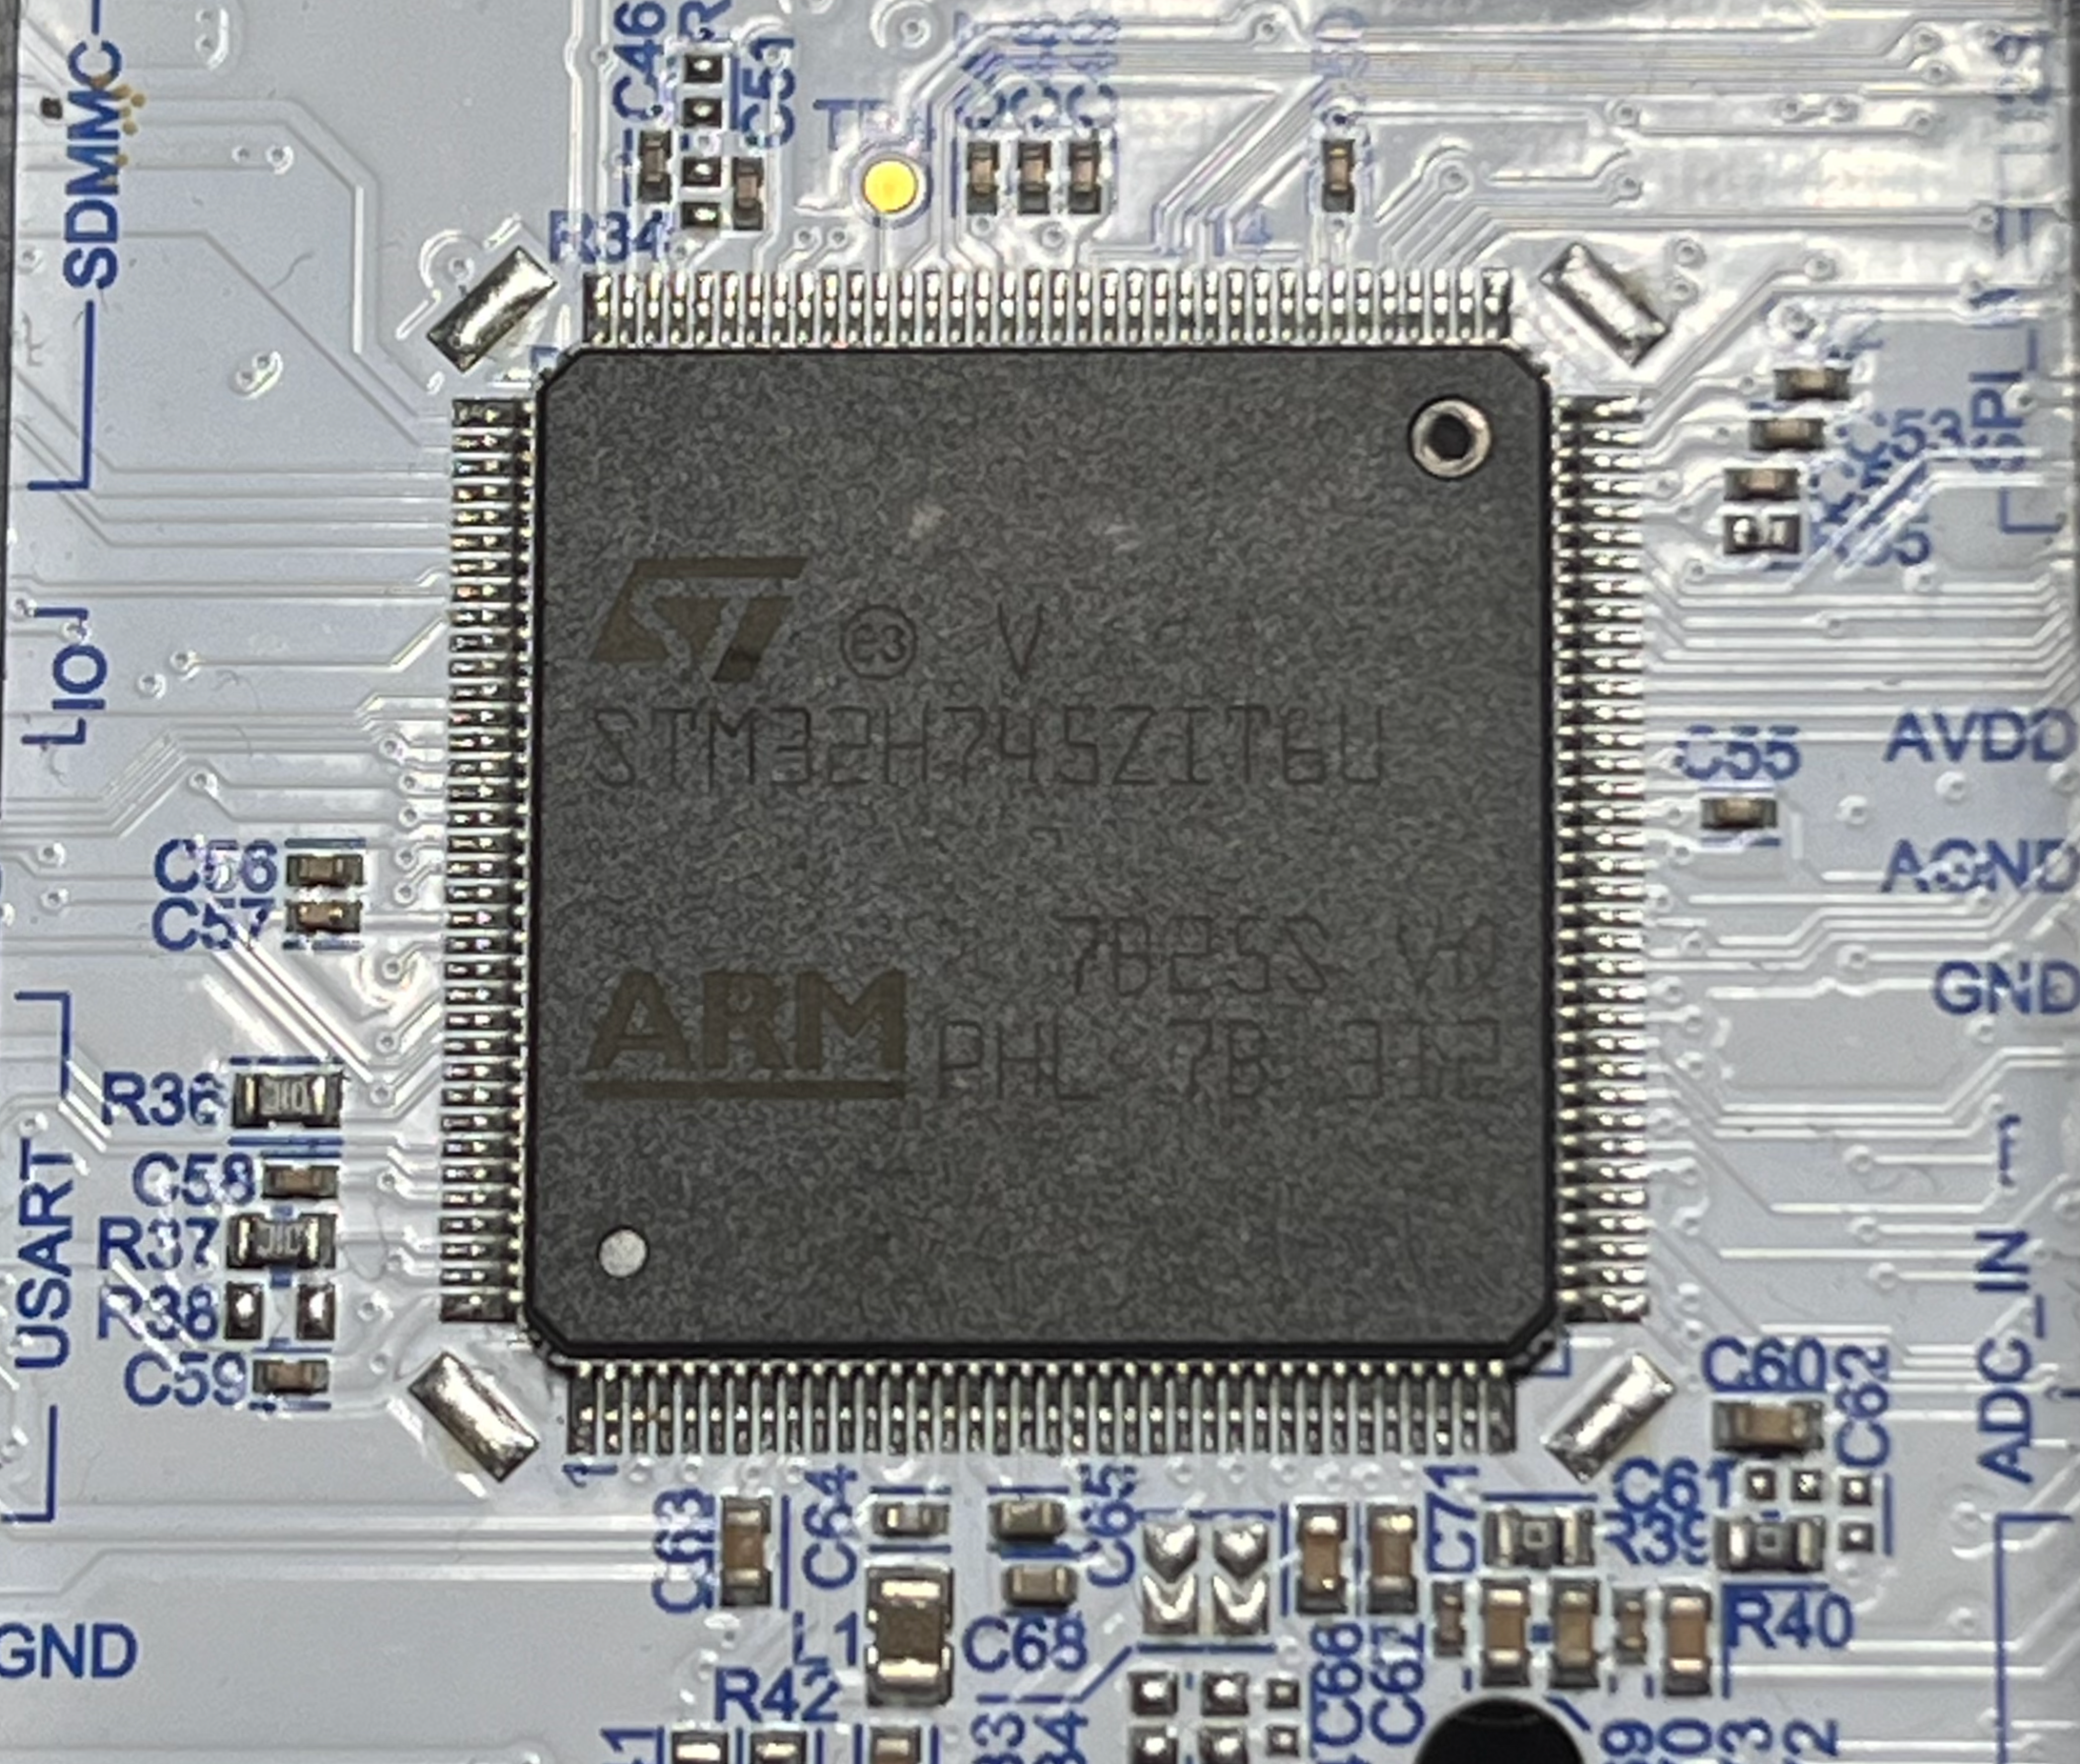
\includegraphics[width=0.5\textwidth]{chapters/Chapter2-HARDWARE/Figures/IMG2-STM32H745ZI-TQ6.png}
    \caption{\textcolor{black}{Il microcontrollore STM32H745ZI-TQ6}}
    \label{fig:etichetta}
\end{figure}

Nel contesto applicativo sono state utilizzate molte delle periferiche poc'anzi citate. Nella successiva sessione si riserverà spazio per approfondire quali di queste e le modalità di utilizzo.
%%%%%%%%%%%%%%%%%%%%%%%%%%%%%%%%%%%%%%%%%%%%%%%%%%%%%%%%%%%%%%%%%%%%%%%%%%%%%%%%%%%%%%%%%%%%%%%%%%%%%%%%%%%%%%%%%%%%%%%%%%%%%%%%%%%%%%%%%%%

%%%%%%%%%%%%%%%%%%%%%%%%%%%%%%%%%%%%%%%%%%%%%%%%%%%%%%%%%%%%%%%%%%%%%%%%%%%%%%%%%%%%%%%%%%%%%%%%%%%%%%%%%%%%%%%%%%%%%%%%%%%%%%%%%%%%%%%%%%%%%%%%%%%%%%%%%%%%%%%%%%%%%%%%%%%%%%%%%%%%%%%%%%%%%%%%%%%%%%%%%%%%%%%%%%%%%%%%%%%%%%%%
%%%%%%%%%%%%%%%%%%%%%%%%%%%%%%%%%%%%%%%%%%%%%%%%%%%%%%%%%%%%%%%%%%%%%%%%%%%%%%%%%%%%%%%%%%%%%%%%%%%%%%%%%%%%%%%%%%%%%%%%%%%%%%%%%%%%%%%%%%%%%%%%%%%%%%%%%%%%%%%%%%%%%%%%%%%%%%%%%%%%%%%%%%%%%%%%%%%%%%%%%%%%%%%%%%%%%%%%%%%%%%%%

\subsection{{NUCLEO-H745ZI-Q. Caratteristiche della scheda}}
La NUCLEO-H745ZI-Q è la scheda di sviluppo (\textit{development board}) che proietta all'esterno tutte le funzionalità del microcontrollore poco fa descritto.
\paragraph{Caratteristiche fisiche}
\begin{itemize}
    \item Dimensioni: $133.34\times 70,00$ [mm].
    \item Peso: 120 [g].
\end{itemize}

\paragraph{ST-LINK/V3E}\mbox{}\\
L'ST-LINK/V3E è un'interfaccia hardware, gestita dal microcontrollore STM32F723, dedicata al collegamento tra elboratore esterno e microcontrollore. Il modulo permette di caricare il compilato \textit{firmware} sul microcontrollore direttamente dalla porta USB Micro-B collegata al sistema di elaborazione.
Il modulo, permette, inoltre, di eseguire il \textit{debug} in tempo reale del codice caricato sull'\textit{MCU}.\\
L'ST-LINK/V3E fornisce anche interfacce ausiliarie utili ai fini dello sviluppo.\\
A seguire un breve elenco esplicativo di queste funzionalità aggiuntive:
\begin{itemize}
    \item VCP (\textit{Virtual COM Port}): lo ST-LINK crea una porta seriale virtuale via USB, in tal modo è possibile collegarsi al microcontrollore come se fosse collegato via UART classica.
    \item MSC (\textit{Mass Storage}): la scheda di sviluppo appare al sistema di elaborazione come una memoria esterna.
\end{itemize}

\paragraph{Alimentazione}\mbox{}\\
La scheda di sviluppo offre diversi approcci per l'alimentazione: 
\begin{itemize}
    \item Alimentazione via USB Micro-B ST-LINK a 5V.
    \item Alimentazione via Jack esterno da 7-12V.
    \item Alimentazione tramite \textit{pin Vin} esterno a 3.3V.
\end{itemize}
Nonostante la presenza di diversi approci di alimentazione e i differenti voltaggi, la tensione di alimentazione del microcontrollore è 3.3V, ottenuta attraverso regolatori interni.\\
Sulla scheda di sviluppo sono presenti dei \textit{jumper}, ovvero dei piccoli interruttori meccanici che permettono di riconfigurare l'\textit{hardware} della scheda evitando di intaccare il \textit{firmware}. Si suggerisce di prestare attenzione alla configurazione 
dei \textit{jumper} qualora si volesse alimentare la scheda da ingressi diversi dal \textbf{COM1} o \textbf{MICRO-B ST-LINK}.\\

\begin{figure}[htbp]
    \centering
    \includegraphics[width=0.6\textwidth]{chapters/Chapter2-HARDWARE/Figures/NUCLELO_DettaglioJumpers.png}
    \caption{NUCLEO-H745ZI-Q. Dettaglio esplicativo dei \textit{jumper}}.
    \label{fig:etichetta}
\end{figure}

\paragraph{Formato fisico}\mbox{}\\
La scheda di sviluppo in esame appartiene alla famiglia \textbf{Nucleo-144} di STMicroelectronics e, dunque, mette a disposizione 2 connettori \textbf{\textit{Morpho}} che espongono i 144 \textit{pin} del microcontrollore. Il sistema di espansione poco fa citato viene chiamato ST Zio.\\
La NUCLEO-H745ZI-Q offre, inoltre, la compatibilità hardware e pinout con gli \textit{Shield Arduino Uno R3}.\\

%%%%%%%%%%%%%%%%%%%%%%%%%%%%%%%%%%%%%%%%%%%%%%%%%%%%%%%%%%%%%%%%%%%%%%%%%%%%%%%%%%%%%%%%%%%%%%%%%%%%%%%%%%%%%%%%%%%%%%%%%%%%%%%%%%%%%%%%%%%
\begin{figure}[htbp]
    \centering
    \includegraphics[width=0.6\textwidth]{chapters/Chapter2-HARDWARE/Figures/IMG1-FotoDaSopraScheda.png}
    \caption{\textcolor{black}{La scheda di sviluppo  NUCLEO-H745ZI-Q}}
    \label{fig:etichetta}
\end{figure}
%%%%%%%%%%%%%%%%%%%%%%%%%%%%%%%%%%%%%%%%%%%%%%%%%%%%%%%%%%%%%%%%%%%%%%%%%%%%%%%%%%%%%%%%%%%%%%%%%%%%%%%%%%%%%%%%%%%%%%%%%%%%%%%%%%%%%%%%%%%

\subsection{NUCLEO-H745ZI-Q. Configurazione ed impiego delle periferiche}
\textcolor{red}{Da inserire una volta sicuri ottenuta la sicurezza delle periferiche hardware}.

% 3) HARDWARE: ALIMENTAZIONE

\input{chapters/Chapter2-HARDWARE/TATTU_LiPo_e_MNR_electronics_PowerSafeModule.tex}
% 4) HARDWARE: MOTORI 

\section{Turnigy AereoDrive SK3-3536 1400KV}
Il Turnigy AereoDrive SK3 3536 1400kv è un motore \textit{Brushless} alimentato a corrente continua e pilotato a trifase con correnti alternate.\\
Il rotore contiene magneti permanenti disposti con polarità alternata lungo la sua circonferenza. Lo statore invece, ospita tre avvolgimenti elettrici (fasi) disposti generalmente a 120 gradi elettrici l'uno rispetto l'altro, connessi ai tre terminali d'uscita che si identificano come A,B e C.\\
Il rotore, essendo formato da magneti permanenti, non necessita di alimentazione: è lo statore a generare il campo magnetico rotante che induce il moto.\\
Il cambio di polarità degli avvolgimenti deve essere gestito da un sistema elettronico esterno, \textit{l'Elettronic Speed Controller (ESC)}, che nella successiva sezione verrà approfondito.\\
I tre conduttori che fuoriescono dal motore rappresentano i terminali delle tre fasi dello statore. Ciascun filo è collegato a uno degli avvolgimenti, e nessuno di essi costituisce un riferimento comune.
Per far ruotare il motore è necessario che tali fasi vengano alimentate secondo una precisa sequenza temporale, generando un campo magnetico rotante. 
Se si dovesse scambiare due dei tre cavi, l'ordine di commutazione si invertirebbe con conseguente variazione del senso di rotazione.\\
Nel progetto sono stati impiegati due motori del tipo precedentemente citato, disposti in configurazione \textbf{controrotante}, con il fine di compensare le rotazioni indesiderate di \textbf{yaw}.
Tale scelta consente di bilanciare le coppie di reazione generate dalle eliche, riducendo il momento torcente sul velivolo. Inoltre, l'adozione di due motori si è resa necessaria in quanto un singolo
attuatore non sarebbe stato in grado di generare una spinta sufficiente a garantire la portanza richiesta dal sistema nelle condizioni operative previste.

\subsection{Turnigy AereoDrive SK3-3536 1400 KV.\@ Caratteristiche fisiche e tecniche:}
\begin{itemize}
    \item Tensione operativa: \textbf{[11.1$\div$16.8] [V]}.
    \item Valore KV: \textbf{1400 $(\frac{RPM}{V})$}.
    \item Potenza massima: \textbf{590 [W]}.
    \item Corrente massima: \textbf{40 [A]}.
    \item Resistenza interna: \textbf{[0.021$\div$0-025] [Ohm]}.
    \item Corrente a vuoto: \textbf{0.021 [A]}.
    \item Diametro dell'albero motore: \textbf{5 [mm]}.
    \item Peso: \textbf{111 [g]}.
    \item Spaziatura fori di montaggio: \textbf{25$\times$25 [mm]}.
    \item Connettori \textit{bullet} \textbf{da 3.5 [mm]}.
    \item Numero dei poli: \textbf{12}.
\end{itemize}

Il valore "KV" è comune nel contesto del modellismo ed indica il numero di giri al minuto (RPM) che il motore compie per ogni \textit{volt} applicato a vuoto, in formula:
\begin{equation}
    RPM = KV\cdot V
\end{equation}
A tensioni di alimentazione maggiori rispetto a quelle specificate il motore rischia di assorbire troppa corrente e surriscaldarsi.\\
I giri al minuto massimi dipenderanno dalla tensione applicata e dalle dimensioni delle eliche.\\
Nel presente progetto, il motore in interesse deve essere alimentato a batteria, vale a dire in corrente continua, lasciando spazio alla necessità di un dispositivo che trasformi la tensione continua erogata dalle batterie in un segnale trifase a corrente alternata.
Il dispositivo in questione è il precedentemente citato \textit{Electronic Speed Controller}.

\begin{figure}[h]
    \centering
    \includegraphics[width=0.5\textwidth]{chapters/Chapter2-HARDWARE/Figures/TurnigyAereoDriveSK3-3536_1400KV.jpg}
    \caption{Turnigy Aereo Drive SK3 3536 1400 KV}
    \label{fig:Hardware drone}
\end{figure}




% 5) HARDWARE: ESC

\section{Turnigy Plush 40A.\@ \textit{Electronic Speed Controller}}
Il Turnigy Plush 40A è un controllore elettronico di velocità per motori \textit{brushless} a corrente continua (BLDC).\\
Trasforma la tensione continua in ingresso in tensioni alternate sfasate di 120 gradi elettrici.\\
L'applicazione della corretta sequenza di correnti alle fasi dello statore richiede la conoscenza della posizione angolare in ogni istante di tempo. Il Turnigy Plush 40A stima tale informazione in maniera indiretta, misurando la forza controelettromotrice indotta dal rotore, evitando così l'uso di sensori di posizione; il dispositivo in interesse può dunque essere definito \textit{sensorless}.
L'E.S.C in questione può essere concettualmente suddiviso in due sezioni principali: la sezione di potenza e la sezione di controllo.
La \textbf{sezione di potenza} è responsabile della conversione \textit{continua-trifase}. Tale conversione è mediata da un ponte trifase a sei MOSFET, suddiviso a sua volta in tre mezzi ponti, ciascuno associato ad una fase del motore.
Ogni mezzo ponte è composto da un trasnistor di alto lato e da un transistor di basso lato, collegati rispettivamente al potenziale positivo della batteria e a massa. L'opportuna commutazione di apertura e chiusura dei sei MOSFET comporta la generazione di un segnale di tensione alternato per ogni fase.\\
La \textbf{sezione di controllo} ha come protagonista un microcontrollore che si occupa della generazione di segnali di pilotaggio e della stima della posizione del rotore. Il microcontrollore riceve in ingresso il comando di velocità di rotazione del motore sotto forma di segnale PWM.
Sulla base di tale comando, il microcontrollore determina il \textit{duty cycle} del PWM e calcola la sequenza di commutazione dei sei MOSFET, con conseguente generazione del campo magnetico rotante dello statore.\\
Il \textit{Double Propeller Ducted Fan} monta due Turnigy Plush 40A, uno per ogni motore.

%%%%%%%%%%%%%%%%%%%%%%%%%%%%%%%%%%%%%%%%%%%%%%%%%%%%%%%%%%%%%%%%%%%%%%%%%%%%%%%%%%%%%%%%%%%%%%%%%%%%%%%%%%%%%%%%%%%%%%%%%%%%%%%%%%%%%%%%%%%%%%%%%%%%%%%%%%%%%%%%%%%%%%%%%%%%%%%%%%%%%%%%%%%%%%%%%%%%%%%%%%%%%%%%%%%%%%%%%%%%%%%%%%%%%
%%%%%%%%%%%%%%%%%%%%%%%%%%%%%%%%%%%%%%%%%%%%%%%%%%%%%%%%%%%%%%%%%%%%%%%%%%%%%%%%%%%%%%%%%%%%%%%%%%%%%%%%%%%%%%%%%%%%%%%%%%%%%%%%%%%%%%%%%%%%%%%%%%%%%%%%%%%%%%%%%%%%%%%%%%%%%%%%%%%%%%%%%%%%%%%%%%%%%%%%%%%%%%%%%%%%%%%%%%%%%%%%%%%%%

\subsection{Turnigy Plush 40A.\@ Caratteristiche fisiche:}
\begin{itemize}
    \item Corrente nominale: 40 [A].
    \item Corrente di picco: 55 [A].
    \item Presenza di un \textit{Battery Eliminator Circuit} (BEC): 5 [V] a 3 [A].
    \item Celle di batteria necessarie per il corretto funzionamento del dispositivo: $[2\div6]$.
    \item Peso: 39 [g].
    \item Dimensioni in [mm]: $60\times24\times15$.
\end{itemize}

\begin{figure}[h]
    \centering
    \includegraphics[width=0.6\textwidth]{chapters/Chapter2-HARDWARE/Figures/TurnigyPlush40A.jpg}
    \caption{Turnigy Plush 40A}
    \label{fig:Hardware drone}
\end{figure}

%%%%%%%%%%%%%%%%%%%%%%%%%%%%%%%%%%%%%%%%%%%%%%%%%%%%%%%%%%%%%%%%%%%%%%%%%%%%%%%%%%%%%%%%%%%%%%%%%%%%%%%%%%%%%%%%%%%%%%%%%%%%%%%%%%%%%%%%%%%%%%%%%%%%%%%%%%%%%%%%%%%%%%%%%%%%%%%%%%%%%%%%%%%%%%%%%%%%%%%%%%%%%%%%%%%%%%%%%%%%%%%%%%%%%
%%%%%%%%%%%%%%%%%%%%%%%%%%%%%%%%%%%%%%%%%%%%%%%%%%%%%%%%%%%%%%%%%%%%%%%%%%%%%%%%%%%%%%%%%%%%%%%%%%%%%%%%%%%%%%%%%%%%%%%%%%%%%%%%%%%%%%%%%%%%%%%%%%%%%%%%%%%%%%%%%%%%%%%%%%%%%%%%%%%%%%%%%%%%%%%%%%%%%%%%%%%%%%%%%%%%%%%%%%%%%%%%%%%%%

\subsection{Turnigy Plush 40A. Programmazione}
Il Turnigy Plush 40A offre la possibilità di programmare il suo comportamento operativo, soddisfando così un vasto spettro di possibili esigenze progettuali.\\
Al fine di ottenere uno specifico comportamento dei motori, tale da adeguarsi alle particolari esigenze di un UAV come il \textit{Double Propeller Ducted Fan}, entrambi gli E.S.C sono stati minuziosamente riprogrammati.\\
L'accesso alla \textit{Programming Mode} e l'effettiva programmazione sono state effettuate mediante l'apposita \textit{Turnigy Programming card}, acquistata separatamente.
Per effettuare la programmazione, è necessario disporre i collegamenti elettrici come in figura:
\begin{figure}[h]
    \centering
    \includegraphics[width=0.6\textwidth]{chapters/Chapter2-HARDWARE/Figures/SchemaCollegamentiProgrammazioneEsc.png}
    \caption{Schema dei collegamenti per la programmazione dell'E.S.C}
    \label{fig: Hardware drone}
\end{figure}\\
La \textit{Turnigy Programming Card} richiede di essere alimentata da un segnale continuo di tensione appartenente al seguente intervallo: $[4.8\div 6] [V]$. Per la navigazione fra i parametri è necessario utilizzare il pulsante \textit{up/down}, mentre, per la selezione dei corrispondenti valori, deve essere utilizzato il pulsante \textit{left/right}.\\
Nel momento in cui verrà selezionato il valore desiderato del parametro in programmazione, il LED  blu, che risponde al nome di \textit{connecting}, lampeggerà, segnalando così il successo dell'operazione.
A seguire, una piccola spiegazione del significato dei parametri e i valori attualmente selezionati:

\paragraph{\small{Brake}}\mbox{}\\
Il parametro \textit{Brake} si riferisce alla modalità con cui viene gestita la mancanza di segnale PWM di controllo. Nel caso in cui dovesse essere impostato ad "ON" il motore verrà immediatamente frenato.\\
Il parametro in analisi non ha grande valenza ai fini progettuali dal momento che qualsiasi prova di volo è stata effettuata nell'apposita gabbia, per cui qualunque combinazione del parametro è accettabile. Nello svolgersi del progetto il parametro è stato impostato ad "OFF". 

\paragraph{\small{Battery Type}}\mbox{}\\
Il \textit{Battery Type} riferisce al dispositivo la tipologia di batteria in utilizzo, questo perché L'E.S.C monitora costantemente la tensione della batteria, quando questa scende sotto una certa soglia, entra in azione il \textit{Low Voltage Cut-off}, riducendo o interrompendo la potenza fornita al motore con il fine di evitare il danneggiamento delle celle.
Diverse tipologie di batterie hanno diverse curve di scarica.
L'E.S.C può gestire solamente due tipologie di batterie, LiPo e NiHM. Il progetto prevede l'utilizzo delle \textbf{Tattu LiPo} perciò il parametro è stato impostato ad Li-xx.

\paragraph{\small{Low Voltage Protection Mode (Cut-off Type)}}\mbox{}\\
Come già riferito in precedenza, la \textit{Low Voltage Cut Off} evita il danneggiamento delle celle delle batterie quando queste scendono sotto una certa soglia impostabile.\\
Il dispositivo permette di scegliere tra \textit{Soft Cut-Off} e \textit{Cut-Off}. Se si dovesse scegliere la modalità \textit{Soft}, al superamento della soglia, l'E.S.C ridurrà gradualmente la potenza in uscita. Se si dovesse, invece, scegliere l'altra modalità, il dispositivo interromperà immediatamente la linea di fornitura di potenza al motore.\\
Al fine di evitare il danneggiamento del sistema, dovuto a un'interruzione improvvisa della fornitura di potenza ai motori durante il volo, seppur all'interno della gabbia, è stata impostata la modalità \textit{Soft Cut-Off}.

\paragraph{\small{Cut Off Voltage}}\mbox{}\\
Il parametro permette di impostare la soglia al di sotto della quale entra in azione la \textit{Low Voltage Protection Mode}.
\begin{itemize}
    \item \textit{Low}: 2.6 [V].
    \item \textit{Medium}: 2.85 [V].
    \item \textit{High}: 3.1 [V].
\end{itemize}
Con il fine di limitare il danneggiamento delle batterie, ottenendo contemporanemante una discreta autonomia di volo, il parametro è stato impostato a \textit{\textbf{Medium}}.\\
Numericamente, considerando le batterie \textbf{Tattu LiPo} a 4 celle, la soglia di attivazione del L.V.C è: $2.85 V\cdot4 = 11.4 V$.

\paragraph{\small{Start Mode}}\mbox{}\\
la \textit{Start Mode} gestisce la modalità di accelerazione del motore da fermo. Sono disponibili tre diverse modalità di partenza, pensate per adattarsi a qualsiasi applicazione.\\
La \textit{Normal Start Mode} costituisce la modalità di accelerazione più reattiva. L'E.S.C applica una rampa di potenza relativamente breve, nel giro di $[0.3\div0.5] [s]$ il motore raggiunge i primi giri utili. L'appena descritta modalità è stata scartata a priori dal momento che, come conseguenza di un'accelerazione repentina, si ha forte stress meccanico sull'albero motore,
inoltre l'improvvisa accelerazione delle eliche può generare forze indesiderate.\\
Nella \textit{Soft Start} la rampa di ingresso è più dolce, di fatti il motore, sotto il controllo dell'E.S.C, impiega $[1\div1.5] [s]$ per arrivare a regime. Infine, nella \textit{Very Soft Start} la potenza viene incrementata nell'arco di $[2\div3] [s]$.\\
Qualsiasi prova di volo del \textit{D.P.D.F} è stata eseguita nell'apposita gabbia di contenimento, in cui il sistema è stato sospeso mediante funi di sostegno, perciò, con il fine di evitare movimenti indesiderati, stress meccanico ed errori di misurazione è stata impostata la \textit{Very Soft Start}.

\paragraph{\small{Timing Mode}}\mbox{}\\
L'E.S.C, con il fine di genesi di rotazione, genera campi magnetici rotanti commutando le tre fasi in sequenza. Le commuttazioni devono avvenire in sincronia con la posizione del rotore. Il \textit{Timing} è l'anticipo angolare con cui l'E.S.C commuta le fasi rispetto alla posizione stimata del rotore.\\
Se il \textit{Timing} dovesse essere basso, il campo magnetico rotante sarebbe quasi allineato con il rotore, disposizione che aumenterebbe l'\textbf{efficienza ellettro-meccanica} complessiva del sistema ma diminuirebbe coppia e velocità. Al contrario, se dovesse essere alto, si avrebbe più potenza e velocità ma anche più dispersione di calore e meno efficienza.\\
L'\textit{High Timing Mode}, a cui corrisponde un anticipo angolare di $[16\div30]^{\circ}$, favorisce potenza e velocità, utile per dispositivi ad alto numero di giri o da corsa. La \textit{Low Timing Mode}, con un'anticipo angolare di $[0\div7]^{\circ}$, garantisce una coppia stabile con minima dispersione di calore con una leggere diminuzione della velocità massima.\\
La \textit{Medium Timing Mode} ($[8\div15]^{\circ}$) costituisce un buon compromesso fra efficienza e prestazioni, dunque è stata scelta ai fini progettali.

\paragraph{\small{Music Li-Po Cells}}\mbox{}\\
La funzionalità è puramente estetica e non influisce sulle prestazioni, per cui non è stata impostata alcuna musica.

\paragraph{\small{Governor Mode}}\mbox{}\\
La \textit{Governor Mode} ha lo scopo di mantenere la velocità di rotazione del motore costante indipendentemente dalle variazioni di carico o tensione della batteria. Non essendo utile ai fini progettuali, il parametro è stato impostato su "OFF".

\begin{figure}[h]
    \centering
    \includegraphics[width=0.6\textwidth]{chapters/Chapter2-HARDWARE/Figures/TurnigyProgrammingCard.jpg}
    \caption{Turnigy Programming Card}
    \label{fig: Hardware Drone}
    \vspace{2mm}
    {\footnotesize L’immagine riportata sopra non è riferita alla configurazione attuale degli ESC, ma ha esclusivamente scopo illustrativo.}
\end{figure}

%%%%%%%%%%%%%%%%%%%%%%%%%%%%%%%%%%%%%%%%%%%%%%%%%%%%%%%%%%%%%%%%%%%%%%%%%%%%%%%%%%%%%%%%%%%%%%%%%%%%%%%%%%%%%%%%%%%%%%%%%%%%%%%%%%%%%%%%%%%%%%%%%%%%%%%%%%%%%%%%%%%%%%%%%%%%%%%%%%%%%%%%%%%%%%%%%%%%%%%%%%%%%%%%%%%%%%%%%%%%%%%%%%%%%
%%%%%%%%%%%%%%%%%%%%%%%%%%%%%%%%%%%%%%%%%%%%%%%%%%%%%%%%%%%%%%%%%%%%%%%%%%%%%%%%%%%%%%%%%%%%%%%%%%%%%%%%%%%%%%%%%%%%%%%%%%%%%%%%%%%%%%%%%%%%%%%%%%%%%%%%%%%%%%%%%%%%%%%%%%%%%%%%%%%%%%%%%%%%%%%%%%%%%%%%%%%%%%%%%%%%%%%%%%%%%%%%%%%%%

\subsection{Turnigy Plush 40A. Risoluzione e controllo dei motori}
\textit{Il Turnigy Plush 40A}, al fine di controllare la velocità di rotazione dei motori, richiede un segnale del tipo PWM alla frequenza tipica del modellismo, vale a dire, $50 [Hz]$.\\
In primo luogo, è necessaria una procedura di armamento dei motori, che consiste nell'invio del segnale PWM con \textit{duty cycle} del $4.75\%$. L'esito dell'operazione di armamento può
essere stabilito mediante delle segnalazioni acustiche emesse dall'E.S.C. A seguire, le emissioni acustiche più comuni:

\paragraph{\small{Attesa di un segnale di armamento valido}}\mbox{}\\
Un'emissione ogni due secondi, segnala l'attesa di un segnale PWM idoneo all'armamento iniziale dei motori. L'emissione viene attivata dal dispositivo immediatamente dopo la connessione di questo all'alimentazione.

\paragraph{\small{Esito positivo dell'operazione di armamento}}\mbox{}\\
Tre emissioni sonore consecutive seguite da un'emissione prolungata, indicano l'esito positivo dell'operazione di armamento.

\paragraph{\small{Esito negativo dell'operazione di armamento}}\mbox{}\\
Una rapida ripetizione di emissioni sonore (una ogni 0.25 [s]) segnala il mancato armamento dei motori, dovuto ad un segnale di ingresso errato. Comunemente l'esito negativo di armamento si può presentare 
nel caso in cui il segnale PWM dovesse avere un \textit{duty cycle} superiore al $4.75 \%$ oppure nel caso in cui il \textit{duty cycle} dovesse repentinamente variare dal $4.75 \%$ a valori superiori.
Si consiglia di attendere $[2\div 6]\, [s]$ prima di iniziare la variazione del \textit{duty cycle} del segnale per il controllo della velocità dei motori.
\\\\
Al seguito di vari accertamenti empirici, è stato stabilito l'intervallo di lavoro dei motori espresso in \textit{duty cycle}: $[6\%\div 12\%]$.

\paragraph{Risoluzione}\mbox{}\\
Quando si tratta di E.S.C, con il termine "risoluzione" non ci si riferisce al numero di campioni di tensione logica distringuibili dal dispositivo, bensì allo "\textit{span}" di valori del \textit{duty cycle} distringuibili.\\
La conoscenza della risoluzione del dispositivo è utile nella determinazione della variazione minima del \textit{duty cycle} del segnale PWM di controllo, che a sua volta permette lo sviluppo di un algoritmo di controllo più efficace.
Per quanto riguarda il \textit{Turnigy Plush 40A}, la documentazione ufficiale non specifica la risoluzione del dispositivo; pertanto, si è fatto riferimento a fonti non ufficili, che indicano una risoluzione compresa trai 8 e 12 bit.\\
Si è optato per uno sviluppo del controllore capace di trascurare la risoluzione del dispositivo, a causa dell'ambiguità di tale informazione.  




%Poiché la batteria fornisce corrente continua e il motore richiede correnti alternate sfasate è indispensabile l'uso di un ESC.\\
%L'ESC trasforma la tensione continua della batteria (14.8 [V] della batteira utilizzata nel progetto) in tensioni alterante sfasate di 120 gradi elettrici. Questo avviene tramite una rete di transistor di potenza (MOSFET) organizzata in un ponte trifase.\\
%L'ESC deve conoscere in ogni istante la posizione angolare del rotore per applicare alla fasi dello statore la sequenza corretta di correnti. L'informazione in questo tipo di applicazioni è spesso stimata indirettamente mediante la misura della forza controelettromotrice indotta dal rotore, evitando l'uso di sensori.\\
%L'ESC riceve un comando esterno (tipicamente un segnale PWM di tipo RC, con impulsi di durata compresa tra 1 [ms] e 2 [ms]). L'ESC agisce da \textit{blackbox} e proporzionalmente al PWM in ingresso modula velocità del motore.\\
%La coppia, e quindi la potenza erogata, dipendono dal duty cycle della modulazione della tensione fornita. 


% 6) HARDWARE: ELICHE

%\section{GEMFAN GF 9060. Eliche}
La corretta realizzazione del progetto dipende anche dalle eliche utilizzate.
% 7) HARDWARE: SERVOMOTORI

% 8) HARDWARE: SENSORE IMU
%%%%%%%%%%%%%%%%%%%%%%%%%%%%%%%%%%%%%%%%%%%%%%%%%%%%%%%%%%%%%%%%%%%%
% TO DO LIST SPIEGAZIONE DEL BOSH SENSORTEC 
% Presentazione del sensore nell'ambito del progetto 
% Presentazione del sensore generale  [OK]
% Principio di misura del sensore: accelerometro, giroscopio e magnetometro [OK]
% Dati tecnici: Dimensioni, peso, alimentaizione, collegamenti, comunicazione 
% Modalità operative del sensore spingendo sulla sensor fusion 

\section{BNO-055 Bosh Sensortec. Unità di misura inerziale e magnetometro}
\textcolor{red}{a cosa serve l'imu in questo progetto?}\\
Il \textbf{BNO-055} è un sensore di orientamento assoluto a 9 assi sviluppato da \textbf{Bosh Sensortec}.
Il dispositivo è un \textit{System in Package}\textcolor{blue}{[A]} che integra un accelerometro triassiale a 14 bit, un giroscopio triassiale a 16 bit, un sensore geomagnetico triassiale e un
microcontrollore Cortex $M0^+$ a 32 bit incaricato nell'eseguire il \textit{software di sensor fusion} integrato.\\
Il \textit{software}, poc'anzi citato, combina i dati provenienti da accelerometro, giroscopio e magnetometro, fornendo: \textbf{Quaternioni, Angoli di Eulero come pitch, roll e yaw e Vettori di orientamento lineari e gravitazionali}.
Nel presente progetto, il \textit{chip} BNO-055 è stato acquistato con montaggio su \textit{scheda di breakout} incluso, dunque nel paragrafo sottostante sono stae aggiunte sia le dimensioni/peso del modulo che le dimensioni/peso del chip.

\subsection{BNO-055 BoshSensortec. Catatteristiche e archiettura}
A seguire una rappresentazione schematica del \textit{System in package BNO-055 Bosh Sensortec}
\begin{figure}[htbp]
    \centering
    \includegraphics[width=0.5\textwidth]{chapters/Chapter2-HARDWARE/Figures/IMG3-Architettura BNO-055.png}
    \caption{\textcolor{black}{Architettura di sistema}}
    \label{fig:etichetta}
\end{figure}



\paragraph{\small{Parametri fisici}}
\begin{itemize}
    \item dimensioni del modulo: $20\times24\times2$ mm.
    \item dimensioni del chip: $3.8\times5.2\times1.1$ mm.
    \item massa del modulo: 3 g.
    \item massa del chip: $\approx 150 mg$.
\end{itemize}

\paragraph{\small{Alimentazione}}\mbox{}\\
Il sensore ha due distinti ingressi di alimentazione:
\begin{itemize}
    \item $V_{DD}$ è il principale \textit{pin} di alimentazione per i sensori interni.
    \item $V_{DDIO}$ è l'ingresso distinto di alimentazione del \textit{$\mu C$} e delle interfacce digitali.
\end{itemize}
Al fine di ottenere una corretta alimentazione per il \textit{System in package} è necessario che l'ingresso $V_{DD}$ sia sotto tensione consigliata prima di alimentare anche l'ingresso $V_{DDIO}$.\\
Il BNO-055 supporta tre differenti modalità di alimentazione: \textit{Normal mode}, \textit{Low power mode} and \textit{Suspend mode}. Per lo sviluppo è stata scelta la modalità \textit{Normal mode}.\\
\small{\textit{Per approdondire le altre modalità, consultare il datasheet: \textcolor{red}{[Riferimento]}}}

\paragraph{\small{Protocolli di comunicazione disponibili}}
\begin{itemize}
    \item $I^2C$.
    \item UART.
    \item SPI.
\end{itemize}
%Anche se lo scrivi sopra nella parte (a cosa serve l'imu a questo progetto rammenta)
\textbf{\textit{\small{Si rammenta che nel presente progetto è stato utilizzato il protoccolo di comunicazione $I^2C$}}}

\subsection{Principio di misura dell'accelerometro, giroscopio e magnetometro}
\paragraph{Accelerometro}\mbox{}\\
L'accelerometro integrato nel BNO-055 Bosh Sensortec è di tipo capacitivo M.E.M.S, \textit{Micro-Eletro-Mechanical System}. Il dispositivo consente la misura dell'accelerazione lungo i tre assi cartesiani.\\
Il principio di funzionamento si basa sulla rilevazione delle variazioni di capacità tra microstrutture mobili e fisse realizzate su un substrato di silicio.\\
L'elemento sensibile di ciascun asse è costituito da una massa sospesa, \textit{proof mass}, vincolata da microtravi elastiche ad una cornice ancorata al substrato. In condizioni di quiete, la massa è in equilibrio e la capacità tra le piastre interdigitate\textcolor{blue}{[A]} rimangono simmetriche.\\
Quando il dispositivo è sottoposto ad un'accelerazione lungo uno degli assi sensibili, la massa inerziale si sposta in direzione opposta a quella dell'accelerazione, generando una variazione differenziale delle capacità tra le piastre.\\
La variazione di capacità viene rilevata da un circuito integrato, che la converte in un segnale elettrico, proporzionale alla velocità applicata.\\
Il segnale analogico prodotto, viene successivamente digitalizzato da un convertirore analogico digitale integrato nel chip.

\paragraph{Giroscopio}\mbox{}\\
Il giroscopio integrato nel dispositivo fa parte della categoria M.E.M.S di tipo vibrante, \textit{vibrating structure gyroscope}, e consente la misura della velocità angolare lungo i tre assi cartesiani.\\
Il principio di funzionamento si basa sull'effetto Coriolis, che si manifesta quando una massa in moto oscillatorio subisce una rotazione rispetto ad un sistema di riferimento inerziale.
All'interno del sensore, ciascun asse dispone di una o più masse vibranti, le quali vengono mantenute in oscillazione a frequenza costante, mediante un circuito di attuazione elettrostatica. Quando il dispositivo ruota attorno ad uno degli assi
la massa subisce una forza di Coriolis data da:
\begin{equation}
    \vec{F_c}=2m(\vec{v}\times \vec{\omega }) 
\end{equation}
dove $m$ è la massa oscillante, $\vec{v}$ è la velocità della massa nella sua traiettoria vibrante, $\vec{\omega}$ è la velocità angolare del corpo.\\
Questa forza induce uno spostamento trasversale rispetto alla direzione di vibrazione, che viene rilevato attraverso variazioni di capacità tra elettrodi fissi e mobili, similmente a quanto avviene nell'accelerometro.\\
Tali variazioni, proporzionali alla velocità angolare, vengono convertite in un segnale elettrico mediante un circuito di lettura differenziale e successivamente digitalizzate tramite un convertitore analogico digitale integrato.

\paragraph{Magnetometro}\mbox{}\\
Il sensore integra inoltre un \textbf{magnetometro ad effetto Hall}, sfruttante il fenomeno fisico della tensione di Hall per misurare l'orientamento del dispositivo rispetto al campo magnetico terrestre.\\
Nella sua forma più semplice, un elemento di Hall è una sottilissima lamina di materiale conduttore o semiconduttore attraversata da una corrente continua controllata. Se su questa lamina agisce un campo magnetico con componente perpendicolare alla direzione della corrente,
i portatori di carica vengono deviati lateralmente della \textbf{forza di Lorentz}:
\begin{equation}
    F = q(\vec{v}\times\vec{B})
\end{equation}
con $\vec{v}$ vettore velocità della carica e $\vec{B}$ vettore campo magnetico. Questa deviazione procude un accumulo di carica ai bordi opposti della lamina, e, in regime stazionario, un campo elettrico trasversale 
che equilibria la forza magnetica. Il risultato è una differenza di potenziale trasversale, la \textbf{tensione di Hall}: $V_H$ che risulta proporzionale alla componente di campo magnetico normale alla superficie del 
sensore e alla corrente che lo attraversa. Per un elmento \textit{Hall} omogeneo abbiamo:
\begin{equation}
    V_H = \frac{I\vec{B_{\perp}}}{nqs}
\end{equation}
dove $\vec{B_{\perp}}$ è la componente del campo perpendicolare al piano della lamina, $n$ la densità di portatori, $q$ il valore di carica elementare e $s$ lo spessore del \textit{film} attivo.
Nel magnetometro ogni elemento di Hall è disposto in modo da avere la propria normale allineata con uno degli assi cartesiani del sistema di riferimento del sensore. Quando il campo magnetico terrestre
attraversa il dispositivo, ciascun elemento rileva la proiezione del vettore $\vec{B}$ lungo il proprio asse, trasformandola in una tensione di Hall proporzionale.\\
Dopo un'opportuna amplificazione della tensione di Hall percepita e una conversione analogico-digitale si ottiene un tripletto di valori numerici che rappresentano le tre componenti cartesiane del campo magnetico locale.\\
Il vettore tridimensionale ottenuto viene ricostruito e poi confrontato con il valore atteso del campo geomagnetico.\\
Attraverso il \textit{sensor fusion}, il magnetometro fornisce quindi il riferimento assoluto per l'\textit{azimut}, vale a dire, la direzione del Nord magnetico rispetto al sistema di riferimento solidale del sensore.

\subsection{Acceletometro, giroscopio e magnetometro}
L'accelerometro, il giroscopio e il magnetometro sono tutti prodotti da Bosh Sensortec.

\paragraph{\small{Accelerometro}}
\paragraph{\small{Giroscopio}}
\paragraph{\small{Magnetometro}}

\paragraph{Modalità operative}\mbox{}\\
Il dispositivo di misura fornisce una grande varietà di segnali di \textit{output}, che possono essere scelti selezziando l'appropiata modalità operativa.\\
Le modalità operative vengono classificate in base all'attivazione o meno del \textit{software di sensor fusion}, nello specifico distinguiamo tra le \textit{Non-Fusion modes} e le \textit{Fusion modes}.

\paragraph{Non-Fusion Modes}
\begin{itemize}
    \item \textbf{ACCONLY}: il dispositivo fornisce solamente dati grezzi di provenienti dall'accelerometro.
\end{itemize}
\textcolor{red}{CONTINUARE DA QUI}



% 9) HARDWARE: SENSORE ALTEZZA
\section{VL53L1X ST. Sensore Time-of-Flight per la misurazione a lunga distanza}
Al fine di ottenere il comportamento desiderato del \textbf{D.P.D.F}, è necessario conoscere la distanza da terra mentre quest'ultimo è in volo.
Bisogna, dunque, includere un sensore apposito.\\
Il \textbf{VL53L1X di STMicroelectronics} è pienamente coerente con i requisiti precedentemente espressi. Tuttavia, non si è optato per l'integrazione
diretta del sensore della casa STMicroelectronics, si è preferito aquistare il modulo \textbf{IRIS11A0J9776} prodotto da \textbf{Pololu}. La \textit{breakout board} di Pololu, contenente
il sensore VL53L1X è stata scelta per semplificare la fase di configurazione elettronica del dispositivo.\\
Per comprendere il suo principio di misura, è opportuno dedicare un'intera sezione alla sua descrizione.

\subsection{Il principio di misura di un sensore \textit{Time-of-flight,ToF}}
La modalità di misura conosciuta come \textit{Time-of-Flight} si basa sulla determinazione del tempo impiegato da un segnale, generalmente un impulso luminoso nella banda dell'infrarosso, per compiere un viaggio
di andata e ritorno tra un emettitore ed un bersaglio riflettente. In particolare, per il dispositivo in analisi, la sorgente di emissione luminosa è costituita da un laser a cavità verticale (VCSEL), che emette 
brevi impulsi di luce modulata. Il segnale emesso si propaga nell'ambiente fino ad incontrare un oggetto. Parte della radiazione viene riflessa e raccolta da un rilevatore sensibile alla luce, generalmente un \textit{SPAD array} o
\textit{"Single-Photon Avalanche Diode"}. Questo rilevatore è in grado di registrare fino all'arrivo di singoli fotoni, consentendo una misura estremamente sensibile del tempo di volo.
Una volta noto l'intervallo temporale tra l'istante di emissione dell'impulso e quello di ricezione del suo \textit{"eco"}, il calcolo della distanza si ottiene applicando la relazione:
\begin{equation}
    d=\frac{c\cdot \Delta{t}}{2}
\end{equation}
dove $d$ è la distanza dell'oggetto dalla superficie, $c$ è la velocità della luce nel vuoto e $\Delta{t}$ è il tempo di volo misurato. Il fattore 2 al denominatore tiene conto che il segnale percorre il tragitto due volte, andata e ritorno.
I "ToF" moderni possono utilizzare tecniche avanzate di correlazione temporale o modulazione di fase per migliorare la precisione e la resistenza al rumore ambientale.\\
Nel caso in esame, il VL53L1X utilizza la tecnologia base ToF o dToF, \textit{"Direct Time-of-Flight"}.

\subsection{VL53L1X STMicroelectronics. Caratteristiche fisiche}
A seguire, un breve elenco delle principali caratteristiche fisiche:
\begin{itemize}
    \item dimensioni del chip: $4.90\times 1.25\times 1.56$ [mm].
    \item dimensioni del modulo: $17.50\times 12\times 2.56$ [mm].
    \item massa del chip: 30 [mg].
    \item massa del modulo: 0.5 [g] (senza i \textit{pin header}).
\end{itemize}

\subsection{VL53L1X STMicroelectronics. Catatteristiche tecniche}
\paragraph{\small{Alimentazione}}\mbox{}\\
Il sensore presenta un unico ingresso di alimentazione il cui nome è $V_{DD}$. L'intervallo di tensione di alimentazione è: \textbf{$[2.6\div 3.5]$ [V]}

\paragraph{\small{Protocollo di comunicazione}}\mbox{}\\
Il dispositvo è stato sviluppato per comunicare con il microcontrollore utilizzando esclusivamente il protocollo di comunicazione $I^2C$. Il sensore dispone della capacità di comunicare in \textit{Fast Mode}, scambiando byte ad una frequenza di 400 [kHz].\\
Il sensore presenta 
\paragraph{\small{XSHUT e GPIO 1 (Interrupt)}}\mbox{}\\
Il VL53L1X dispone di un ingresso denominato \textbf{XSHUT}, che consente di spegnere o riavviare il dispositivo a livello \textit{hardware}, indipendentemente dall'\textit{Host}.
Portando l'ingresso al livello logico basso, il sensore entra in modalità di \textit{shutdown}, interrompendo le misurazioni e riducendo il consumo di corrente. Al contrario, appliccando
un livello di tensione alto, il sensore viene inizializzato e reso operativo.\\
Oltre che l'ingresso \textbf{XSHUT}, il sensore dispone di un'\textbf{uscita} denominata \textbf{GPIO1}, spesso indicata anche come \textbf{INT (interrupt)}, la cui funzione principale è segnalare al microcontrollore 
eventi o stati del sensore.\\
Nel presente progetto, il pin XSHUT è stato utilizzato esclusivamente per il \textit{reset} forzato del sensore, mentre il GPIO1 è stato impiegato per segnalare la disponibilità della misura,
semplificando il firmware, riducendo il cairico computazionale e consentendo la gestione della temporizzazione, aspetti che verrano approfonditi nella dedicata sezione nel capitolo \textit{Software}.

\paragraph{\small{Emettitore}}\mbox{}\\
Il \textit{VL53L1X} monta un emettitore \textbf{laser ad infrarossi di \textit{classe uno}}. Quest'ultimo fa riferimento alla classificazione di sicurezza stabilita dalla norma internazionale \textbf{IEC 60825-1}.
La classificazione ha il dovere di descrivere quanto un emissione laser possa essere pericolosa per l'interazione umana (occhi, pelle ecc). La normativa organizza gli emettitori in \textit{classi}, dove 
ogni classe rappresenta un livello crescente di rischio. Per un Laser di \textit{classe uno}, come quello emesso dal dispositivo, le condizoni operative normali, sono considerate sicure per occhi e pelle.

\paragraph{\small{Field of View  (FoV)}}\mbox{}\\
Il \textit{Field of View} è l'angolo massimo entro il quale il dispositivo rileva un oggetto. Per quanto riguarda l'emettitore in esame, il \textbf{FoV} è all'incirca di \textbf{$27\degree$}.\\
A seguire, un'immagine esplicativa del \textit{FoV}:
\begin{figure}[h]
    \centering
    \includegraphics[width=0.9\textwidth]{chapters/Chapter2-HARDWARE/Figures/cone.jpg}
    \caption{Field of View del VL53L1X}
    \label{fig:Hardware drone}
\end{figure}

%%\input{chapters/Appendice e Approfondimenti/Appendice.tex}
\input{chapters/Chapter2-HARDWARE/chapter2-TUTORIAL.tex}
\input{chapters/chapter1-TUTORIAL/chapter1.tex}
%\chapter{Traduzione articolo professore}
\section{Introduzione}
Al giorno d’oggi, la nostra qualità della vita dipende sempre più dai sistemi infrastrutturali, i quali influenzano la società contemporanea fornendo ogni tipo di bene. Tuttavia, queste infrastrutture stanno invecchiando e, per evitare guasti o problemi più gravi, è necessario affrontare diverse problematiche nelle procedure di manutenzione.
Purtroppo, l’elevato costo, unito alla difficoltà per gli operatori umani di raggiungere i luoghi di intervento (specialmente considerando gli aspetti legati alla sicurezza), costituiscono forti limiti all’applicazione reale. Per questa ragione, i ricercatori hanno esplorato nuove modalità per automatizzare le procedure di ispezione [1] e, attualmente, la maggior parte degli Unmanned Aerial Vehicles (UAV) proposti per supportare le ispezioni infrastrutturali sono droni [2], [3].

Nonostante le soluzioni innovative, persistono ancora importanti limitazioni da superare: queste vanno dal miglioramento delle prestazioni dei sistemi robotici [4], [5] fino alle problematiche cooperative e di sicurezza [6], [7]. I limiti principali nei compiti di ispezione riguardano innanzitutto le eliche dei droni, poiché sono pericolose e inadatte alle ispezioni non distruttive a contatto. Inoltre, quando questi UAV vengono impiegati in compiti cooperativi con l’essere umano, è necessaria un’interazione sicura, che non può essere garantita dai droni convenzionali.

Un’ulteriore sfida consiste nel controllo preciso di questi robot a base flottante: in molti casi è richiesta un’elevata precisione e, attualmente, per ottenere buona stabilità, si ricorre a soluzioni con più eliche, a discapito dei costi elevati.

In questo lavoro si affrontano questi limiti presentando un’architettura alternativa di UAV denominata Double Propeller Ducted-Fan (DPDF), considerata vantaggiosa per le ispezioni sicure e l’interazione uomo-macchina.

Il primo prototipo simile di Ducted-Fan è stato studiato per la prima volta nel 1997 [8], e successivamente in [9], [10], [11], [12]. In tali studi, l’architettura dell’UAV prevedeva una singola elica ed era utilizzata per analizzare rapide transizioni nelle manovre di volo.

Il lavoro più recente presentato in [9] si compone di due elementi principali:

una singola elica a passo fisso che genera la spinta principale,
due livelli di superfici aerodinamiche attuate (flap), che, agendo con il flusso dell’elica principale, forniscono le componenti di forza e coppia necessarie per ottenere la piena controllabilità dell’assetto.
L’architettura proposta in questo articolo può essere impiegata in diverse attività di ispezione infrastrutturale in condizioni di sicurezza, ed è in grado di interagire con esseri umani evitando collisioni pericolose. Inoltre, può essere dotata di sensori e funzionalità di intelligenza artificiale per migliorarne l’autonomia e l’evitamento degli ostacoli.
Il DPDF è illustrato nella Figura 1: a differenza dell’approccio con due livelli di flap, esso utilizza due eliche controrotanti per contrastare la coppia di reazione generata dal momento giroscopico introdotto dall’elica. Questa soluzione consente anche di governare separatamente la dinamica dell’imbardata (yaw). Inoltre, con questa nuova configurazione, è necessario un solo livello di flap per controllare l’assetto e stabilizzare il volo.

La letteratura sul tema dei Ducted-Fan si è evoluta in diverse direzioni, e solo un altro studio [13] presenta un’idea architetturale simile. Tuttavia, in [13], [14] non vengono forniti tutti i dettagli costruttivi e parametri, e soprattutto il modello dinamico proposto è differente da quello sviluppato nel presente lavoro. In particolare, [13] utilizza un modello semplificato assumendo che la velocità angolare di imbardata sia nulla, mentre in questo studio tale assunzione viene superata.

È stata progettata una tecnica di controllo lineare che separa il controllo di posizione da quello dell’assetto, ottenendo prestazioni incoraggianti; al contrario, in letteratura per UAV simili le tecniche lineari non riescono a raggiungere gli stessi risultati [15].

La validità dell’intero modello e dello schema di controllo è stata valutata testando la tecnica di controllo lineare sul modello non lineare, considerando disturbi del vento e rumori dei sensori in simulazione. Le simulazioni sono state eseguite nell’ambiente Matlab Simulink e i risultati incoraggianti rappresentano il primo passo verso lo sviluppo di un prototipo attualmente in costruzione da parte degli autori.

%%%%%%%%%%%%%%%%%%%%%%%%%%%%%%%%%%%%%%%%%%%%%%%%%%%%%%%%%%%%%%%%%%%%%%%%%%%%%%%%%%%%%%%%%%%%%%%%%%%%%%%%%%%%%%%%%%%%%%%%%%%%%%%%%%%%%%%%%%%%%%%%%%%%%%%%%%%%%%%%%%%%%%%%%%%%%%%%%%%%%%%%%%%%%%%%%%%%%%%%%%%%%%%%%%
%%%%%%%%%%%%%%%%%%%%%%%%%%%%%%%%%%%%%%%%%%%%%%%%%%%%%%%%%%%%%%%%%%%%%%%%%%%%%%%%%%%%%%%%%%%%%%%%%%%%%%%%%%%%%%%%%%%%%%%%%%%%%%%%%%%%%%%%%%%%%%%%%%%%%%%%%%%%%%%%%%%%%%%%%%%%%%%%%%%%%%%%%%%%%%%%%%%%%%%%%%%%%%%%%%
%%%%%%%%%%%%%%%%%%%%%%%%%%%%%%%%%%%%%%%%%%%%%%%%%%%%%%%%%%%%%%%%%%%%%%%%%%%%%%%%%%%%%%%%%%%%%%%%%%%%%%%%%%%%%%%%%%%%%%%%%%%%%%%%%%%%%%%%%%%%%%%%%%%%%%%%%%%%%%%%%%%%%%%%%%%%%%%%%%%%%%%%%%%%%%%%%%%%%%%%%%%%%%%%%%

\section{Modello del DPDF}
In questa sezione vengono brevemente introdotti i parametri cinematici e le equazioni dinamiche proposte per il sistema. Sono stati considerati due sistemi di riferimento (Fig. 1):

\begin{itemize}
  \item \textbf{I} è il sistema di riferimento inerziale, associato alla Terra: l'asse $X_i$ punta verso Nord, $Y_i$ verso Est e $Z_i$ verso il centro della Terra. Il sistema di riferimento è rigidamente vincolato ad essa ed è definito come $\Sigma_i = \{O_i, \vec{i}_i, \vec{j}_i, \vec{k}_i\}$.
  \item \textbf{B} è il sistema solidale al corpo (Body Frame), riferito al DPDF: l'asse $X_b$ punta in avanti, $Y_b$ verso destra e $Z_b$ verso il basso. Il centro del sistema è posto nel baricentro del DPDF, ed è definito come $\Sigma_b = \{O_b, \vec{i}_b, \vec{j}_b, \vec{k}_b\}$.
\end{itemize}

Nel testo, il vettore $x$ espresso nel sistema inerziale è indicato con $^i x$, mentre nel sistema solidale al corpo è indicato con $^b x$.

Per ricavare un modello matematico, è stato utilizzato l’approccio di Newton-Eulero per il moto dei corpi rigidi. In particolare, il modello dinamico dell’UAV rispetto al sistema inerziale è descritto dalle seguenti equazioni del moto:

\begin{equation}
m \, \ddot{\vec{p}}^{\, i} = \mathbf{R}^{i}_{b} \, \vec{F}^b
\end{equation}
\begin{equation}
\mathbf{I}_G^b \, \dot{\vec{\omega}} = -\mathbf{S}(\vec{\omega})^b \, \mathbf{I}_G^b \, \vec{\omega} + \vec{\tau}^b
\end{equation}

\noindent Dove:
\begin{itemize}
  \item $\vec{p} = (x, y, z)^T$ rappresenta la posizione del centro di massa,
  \item $m$ è la massa totale del veicolo,
  \item $\mathbf{R}^{i}_{b}$ è la matrice di rotazione dal sistema corpo al sistema inerziale (parametrizzata dagli angoli di rollio $\phi$, beccheggio $\theta$ e imbardata $\psi$),
  \item $\vec{F}^b$ e $\vec{\tau}^b$ sono rispettivamente il vettore delle forze e delle coppie espresse nel sistema corpo.
\end{itemize}

La matrice antisimmetrica $\mathbf{S}(\vec{\omega})$ è costruita a partire dalla velocità angolare $\vec{\omega}$ come segue:

\begin{equation}
\mathbf{S}(\vec{\omega}) =
\begin{bmatrix}
0 & -\omega_z & \omega_y \\
\omega_z & 0 & -\omega_x \\
-\omega_y & \omega_x & 0
\end{bmatrix}
\end{equation}

\subsection{Equazioni del moto}

Le equazioni di cinematica sono espresse nel sistema inerziale (I), mentre quelle dinamiche nel sistema corpo (B). Le variabili $\dot{x}_G, \dot{y}_G, \dot{z}_G$ rappresentano le velocità lineari nel sistema I, mentre $\dot{u}, \dot{v}, \dot{w}$ rappresentano le accelerazioni lineari nel sistema B. Le derivate $\dot{\phi}, \dot{\theta}, \dot{\psi}$ sono le velocità angolari rispetto al sistema I, mentre $\dot{\omega}_x, \dot{\omega}_y, \dot{\omega}_z$ sono le accelerazioni angolari rispetto agli assi del sistema B.

Tutti i parametri fisici usati nel modello sono riportati nella Tabella I. In particolare:
\begin{itemize}
  \item $k_N$: coefficiente della coppia resistente aerodinamica,
  \item $k_T$: costante di spinta,
  \item $k_\text{flap}$: parametro che raccoglie vari coefficienti legati ai flap (verrà spiegato in dettaglio nella sottosezione successiva).
\end{itemize}

Questi valori sono stati scelti in base al prototipo attualmente in costruzione.

\paragraph{Equazioni cinematiche (sistema inerziale):}
\begin{align}
\dot{x}_G &= w(\sin\phi \sin\psi + \cos\phi \cos\psi \sin\theta) - v(\cos\phi \sin\psi - \cos\psi \sin\phi \sin\theta) + u\cos\psi \cos\theta \\
\dot{y}_G &= v(\cos\phi \cos\psi + \sin\phi \sin\psi \sin\theta) - w(\cos\psi \sin\phi - \cos\phi \sin\psi \sin\theta) + u\cos\theta \sin\psi \\
\dot{z}_G &= w\cos\phi \cos\theta - u\sin\theta + v\cos\theta \sin\phi
\end{align}

\paragraph{Equazioni dinamiche (sistema corpo):}
\begin{align}
\dot{u} &= \omega_z v - \omega_y w - g \sin\theta \\
\dot{v} &= -\omega_z u + \omega_x w + g \cos\theta \sin\phi \\
\dot{w} &= \omega_y u - \omega_x v - \frac{T}{m} + g \cos\theta \cos\phi
\end{align}

\begin{align}
\dot{\omega}_x &= \frac{1}{I_{xx}}(\omega_z \omega_y - k_{\text{flap}} b T) \\
\dot{\omega}_y &= \frac{1}{I_{yy}}(\omega_x \omega_z (I_{zz} - I_{xx}) + k_{\text{flap}} a T) \\
\dot{\omega}_z &= \frac{1}{I_{zz}}(\omega_x \omega_y (I_{xx} - I_{yy}) + \frac{k_N}{k_T} c)
\end{align}

\begin{align}
\dot{\phi} &= \omega_x + \omega_y \sin\phi \tan\theta + \omega_z \cos\phi \tan\theta \\
\dot{\theta} &= \omega_y \cos\phi - \omega_z \sin\phi \\
\dot{\psi} &= \omega_y \frac{\sin\phi}{\cos\theta} + \omega_z \frac{\cos\phi}{\cos\theta}
\end{align}

%%%%%%%%%%%%%%%%%%%%%%%%%%%%%%%%%%%%%%%%%%%%%%%%%%%%%%%%%%%%%%%%%%%%%%%%%%%%%%%%%%%%%%%%%%%%%%%%%%%%%%%%%%%%%%%%%%%%%%%%%%%%%%%%%%%%%%%%%%%%%%%%%%%%%%%%%%%%%%%%%%%%%%%%%%%%%%%%%%%%%%%%%%%%%%%%%%%%%%%%%%%%%%%%%%
%%%%%%%%%%%%%%%%%%%%%%%%%%%%%%%%%%%%%%%%%%%%%%%%%%%%%%%%%%%%%%%%%%%%%%%%%%%%%%%%%%%%%%%%%%%%%%%%%%%%%%%%%%%%%%%%%%%%%%%%%%%%%%%%%%%%%%%%%%%%%%%%%%%%%%%%%%%%%%%%%%%%%%%%%%%%%%%%%%%%%%%%%%%%%%%%%%%%%%%%%%%%%%%%%%
%%%%%%%%%%%%%%%%%%%%%%%%%%%%%%%%%%%%%%%%%%%%%%%%%%%%%%%%%%%%%%%%%%%%%%%%%%%%%%%%%%%%%%%%%%%%%%%%%%%%%%%%%%%%%%%%%%%%%%%%%%%%%%%%%%%%%%%%%%%%%%%%%%%%%%%%%%%%%%%%%%%%%%%%%%%%%%%%%%%%%%%%%%%%%%%%%%%%%%%%%%%%%%%%%%

\section{Disturbi}

Durante le simulazioni, sono stati considerati i disturbi comuni che si manifestano nelle condizioni reali di volo. Per ottenere un buon controllo del velivolo, è essenziale misurare l’assetto dell’UAV rispetto a un sistema di riferimento inerziale. Questa misurazione richiede sensori in grado di rilevare l’orientamento del veicolo—tra i quali l’IMU (Unità di Misura Inerziale), ampiamente utilizzata in diversi ambiti, dai droni alla locomozione umana \cite{16}, fino ai sistemi di sicurezza attiva nei veicoli \cite{17,18}. Come tutti i sensori, anche l’IMU è soggetta a disturbi.

%\paragraph{1 Disturbi dell’IMU:} i ben noti svantaggi di questo sensore includono il rumore sulle misure grezze e l’**errore di integrazione** che si accumula quando il sistema di guida integra continuamente le accelerazioni nel tempo per calcolare velocità e posizione. Tali errori sono introdotti nel sistema durante le simulazioni. In dettaglio:
%\begin{itemize}
 % \item Si è considerata una densità spettrale di potenza (PSD) pari a $400 \mu g/\( \sqrt{\mathrm{Hz}} \)$ sulle variabili misurate $(\(\ddot{x}, \ddot{y}, \ddot{z}\))$, che vengono integrate due volte nel loop di retroazione per ottenere le posizioni $(x, y, z)$.
  %\item Analogamente, per simulare il rumore dei giroscopi, si è utilizzato l’RMS del rumore di 0,05\°/s (dalla scheda tecnica), convertito in PSD seguendo la formula \( \mathrm{PSD} = \mathrm{RMS}^2 \, T_c \), dove \( T_c \) è il tempo di campionamento. I rumori dei giroscopi agiscono sulle misure \(\dot{\omega}_x, \dot{\omega}_y, \dot{\omega}_z\).
%\end{itemize}

Un approccio valido per filtrare tali rumori è stato esplorato in \cite{16} e potrebbe essere implementato e testato in futuri sviluppi.

\paragraph{2 Disturbi del vento:} un’ulteriore fonte di disturbo per i velivoli è rappresentata dall’effetto del vento. Per modellare tali disturbi, comunemente si considerano vari approcci a seconda della superficie colpita. Poiché le eliche del DPDF sono protette dalla struttura esterna, si può assumere che il vento impatti principalmente su quest’ultima. Inoltre, la modellazione del vento risulta più semplice in quanto le forze e le coppie agiscono sulla struttura e non direttamente sulle eliche.

Seguendo l’approccio proposto in \cite{19}, dove il vento è considerato quasi costante, in questo lavoro si è adottata una simulazione in cui i disturbi del vento sono una funzione variabile nel tempo anziché costante, al fine di meglio emulare le condizioni reali ( \( v_x(t), v_y(t) \) ). Tali effetti introducono disturbi nelle velocità, mentre gli effetti sull’assetto sono trascurabili—dato il design con eliche ducted.

Alla luce di ciò, il modello può essere riscritto includendo tutti i disturbi additivi considerati:
\[
\dot{\mathbf{x}}_s = A \mathbf{x}_s + B u(t) + \mathbf{d}
\]
dove il vettore dei disturbi è:
\[
\mathbf{d} = \bigl( v_x,\, v_y,\, 0,\, \dot{d}_u,\, \dot{d}_v,\, \dot{d}_w,\, \dot{d}_{\omega_x},\, \dot{d}_{\omega_y},\, \dot{d}_{\omega_z},\, 0,\, 0,\, 0 \bigr)^T
\]





%%%%%%%%%%%%%%%%%%%%%%%%%%%%%%%%%%%%%%%%%%%%%%%%%%%%%%%%%%%
%                   Back matter contents
%%%%%%%%%%%%%%%%%%%%%%%%%%%%%%%%%%%%%%%%%%%%%%%%%%%%%%%%%%%
\backmatter

%\bibliographystyle{IEEEbib}
%\bibliography{IEEEabrv,bibliografia}

\bibliographystyle{unsrt}
\bibliography{frontbackmatters/bibliography.bib}

\end{document}
